
\Section{Introduction}
Although blockchain and other types of distributed ledgers are still in their infancy a growing number of people and companies are starting to see that they hold great promise, especially when it comes to financial technology, where things like trust and security is held to be very important. 

%https://nordic.businessinsider.com/bitcoin-history-cryptocurrency-satoshi-nakamoto-2017-12?r=US&IR=T
%https://bitcoin.org/bitcoin.pdf
%https://www.blockchain.com/sv/btc/block-height/0
%https://www.theverge.com/2013/5/6/4295028/report-satoshi-nakamoto
%bloody: https://bitcointalk.org/index.php?topic=234.msg1976#msg1976
%https://pastebin.com/syrmi3ET

%There is alot more things that could be writen here. speculations on who satoshi is, previous bitcoin like projects, why he diapeared etc...
\Subsection{The origins of bitcoin}
The most well known, developed and researched blockchain technology is know as Bitcoin. The mysterious nature of bitcoins creator makes hard to pinpoint how and when the idea was first thought up and when the development started, the most exact way and most well known would be to pinpoint at: \texttt{2009-01-03 18:15:05}, which is the timestamp on the very first block in the bitcoin blockchain, however the white paper (\textbf{Bitcoin: A Peer-to-Peer Electronic Cash System}) specifying the technical details circulated on cryptographic mailing lists as early as 31 October 2008, and the domain name \texttt{bitcoin.org} was registered 18 August 2008. 

\Subsubsection{Satoshi Nakamoto}

The author name given in the white paper is \textbf{\texttt{Satoshi Nakamoto}}, this name is believed to be a pseudonym. Satoshi remained in the bitcoin community for a couple of years. Regularly posting on the forum \texttt{bitcointalk.org} and keeping up with conversations in the mailing list. Those who have been interested in finding out Satoshi's real identity have analyzed his active time and language used. The findings were that Satoshi was most active during Western European day time, and he also used a lot of Anglo-colloquialisms such as ''bloody hard'', and ''flat'' instead of apartment, so a popular theory is that Satoshi lived in Britain at least during this time. 

\texttt{April 23, 2011} was the last time anyone ever heard from Satoshi Nakamoto, in a mail to a fellow developer Mike Hearn he said ''I've moved on to other things.  It's in good hands with Gavin and everyone.''. Speculations on who Satoshi really is still going strong even to this day, but Nakamoto's true identity is so far unknown. 

\Subsection{Basics on Bitcoin}
Most people, even the layman with no blockchain experience, have at least heard of bitcoin. But the exact details of how it works is not common knowledge. Described in a single sentence: bitcoin is a currency where a communal ledger that is shared between the whole world. The ledger holds the information on who owns what in terms of money or other assets. The regular monetary system we are used to has a centralized authority, for example a central bank, who decides how much money is in circulation, who can transact with who etc. The monetary system presented by bitcoin has no centralized authority, instead it relies on decentralized, trust-less verification.

These usually are the main concerns people have with distributed ledgers:
\begin{itemize}
	\item How is spending someone else's money prevented?
	\item How is spending the same money in different places in the world prevented?
	\item How is the consensus on the order of transactions reached?
	\item How do I interact with it?
	\item What type of transactions can you make?
\end{itemize}

These questions will be given ansers in the sections below.

%http://www.secg.org/sec2-v2.pdf
%https://en.bitcoin.it/wiki/Secp256k1
%Mastering bitcoin
% More could be writen on why a signature could not be forged
% More on how secure 256 bit is
\Subsubsection{Digital signatures}
Bitcoin would not be possible at all without the underlying cryptographic mathematics. When it comes to proving ownership in bitcoin ECDSA (Elliptic curve digital signature algorithm) is used. Elliptic curve cryptography will not be covered in depth here but the basic idea is that you have a private and public key. The public key can be shared with anyone without danger, the public key can be derived from the private key, but not the other way around, this is something called trap-door mathematics. This means that it is easy to go one way via equations. But going back is nearly impossible. The reason for it not being completely impossible is because any potential attacker could always just keep guessing private keys until the right one is found. However with a sufficiently large private key it should take several million years to find the correct private key even with unrealistically strong and fast computers. 

The most common transaction made on the blockchain is one where you ''pay to'' a public key. Who ever holds the private key paired with that public key can then via a mathematical equation prove that they hold the private key without actually revealing the private key.

\begin{figure}[H]
	\centering
	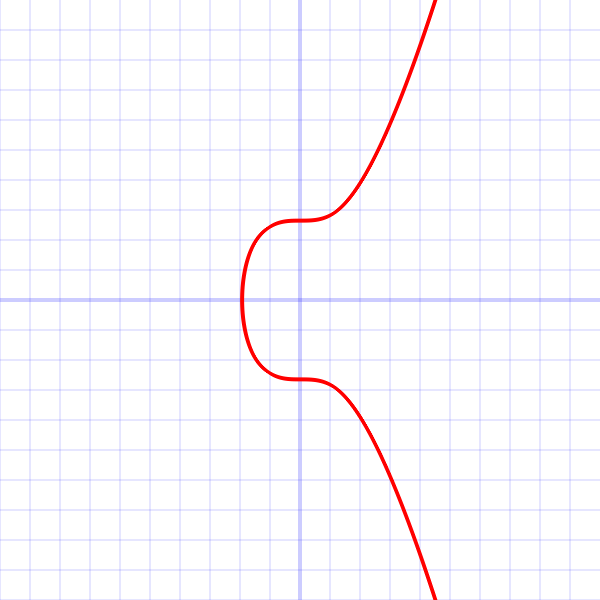
\includegraphics[width=0.5\textwidth]{introduction/images/Secp256k1.png}
	\caption{The \texttt{Secp256k1} plotted over real numbers. Note that the real curve is over a field, and thus looks more like a scattering of random points}
	\label{fig:eccbasic}
\end{figure}

The elliptic curve used can hold different parameters that defines it, certain elliptic curves are standardized and have their own names. The curve used in bitcoin is named \texttt{Secp256k1}.

%Mastering bitcoin
\Subsubsection{Blocks and the blockchain}
A block is fairly simple to understand, it is simply a datatype or structure that holds information about it self, all the transactions that can fit and the previous block in the chain (more on that in a bit). Because every block holds information about the previous block you can follow all blocks backwards in time all the way back to the original, alos called the genesis block. This is what is referred to as the blockchain. 

A block could be added to the chain by anyone in the world. However it will only be accepted if it has sufficient proof of work, and this is the key to how consensus is reached in the network 

\begin{figure}[H]
	\centering
	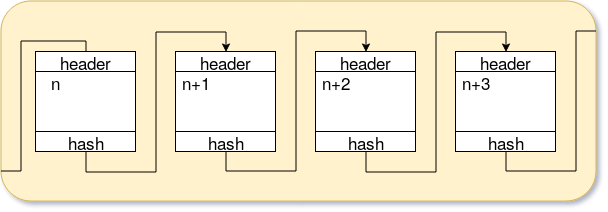
\includegraphics[width=0.5\textwidth]{introduction/images/blockchain.png}
	\caption{A basic overview of a blockchain}
	\label{fig:blockchain}
\end{figure}

%The section on SHA256 can be improved
\Subsubsection{Proof of work}
Proof of work is, just like the digital signatures, based in cryptographic mathematics. Before we go on you first need to understand what a hashing algorithm does, the hashing algorithm used in bitcoin is called \texttt{SHA256}. \texttt{SHA256} takes in data of any size and produces a sort of finger print of 256 bits. 

For example the \texttt{SHA256} of the text ''cool'': 

\fbox{\begin{minipage}{15em}
	\texttt{echo "cool" | openssl sha256}
\end{minipage}}

Produces: 

\fbox{\begin{minipage}{\textwidth / 2 - 1em}
		\texttt{27c16ce7e3861da034af1bb356d6a4f38cb84fa\\65d51fa62f69727143b4c6b60}
\end{minipage}}

The text produced is actually bytes represented in a hexadecimal number system, in fact the entire string can be considered to be a very large number. Just like with the digital signature there is no known viable way that can take a hash and find what the original data that produced it was. 

There is a term in bitcoin called mining difficulty, or just difficulty. This is a large number, 256 bits to be exact. When you want to add a new block to the chain you have to do something called mining, this is a process where you change certain variables in the block until the hash of the block header (Think of this a number) is less than the target difficulty. The term hashpower refers to how many times the machine you are using to mine blocks can test a certain combination of variables per second, or H/s.

The difficulty of mining a block is adjusted about every 2 weeks. The difficulty is so that the combined hashpower of the entire world is enough to mine one block every 10 minutes on average. 

The accepted order of transactions is the order going backwards from the latest block on the longest chain. The longest chain is always the one that the majority is mining towards. This is simplified to the extreme but what it basically means is that as long as you trust 51\% of the participants in the network you can also trust that the order of transactions is correct. This mechanism prevents things like double spending the same money and holds a property called emergent consensus, which means that eventually the entire netowrk will agree on the order of transactions.

In figure \ref{fig:blockchain2} is a diagram showing the longest chain, meaning the chain with most proof of work. The block in green is the latest block on that chain. The yellow block is what is known as a stale block, a block that is part of the chain but not part of the longest chain of blocks. Transactions in a stale block are not considered valid, and eventually they can be pruned (deleted) because they do not effect the future in any way. A stale block occurs if a new block is found in different parts of the network at almost the same time. Then the network will be split, each node tries to find the next block on the chain of whatever block they received first. In the case shown below the chain on the left ''won'' and the green block is now the longest chain.

The red block in figure \ref{fig:blockchain2} is what is known as an orphan block, that is it has no known parent in the chain. This can happen if someone mines a block that is malformed or when building the chain for a new node and the blocks are received out of order.

\begin{figure}[H]
	\centering
	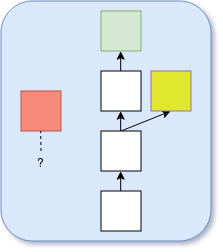
\includegraphics[width=0.2\textwidth]{introduction/images/more_blockchain.png}
	\caption{A diagram showing the longest chain, The green block is the latest block on the longest chain. The red block is a an orphan block, the yellow block is a stale block}
	\label{fig:blockchain2}
\end{figure}


\Subsubsection{Software}
Just like how you can use regular money without knowing the underlying process and technology of for example the banking system, you can use bitcoin with out knowing the details of how it works. There is plenty of software that handles wallets transactions etc for you. 

\Subsubsection{Programmable transactions}
Bitcoin has another feature that makes it very versatile in what it can do and that is that every transaction is programmable. As mentioned earlier the most common transaction is sending the money to someones public key. What really goes on here is that the person who wants to spend whatever money was sent to them has to prove programmatic that they own the private key related to that public key. 

This is not the only type of transaction possible, bit con has it's own little programming language called \texttt{Script}. Any type of transaction that can be described in script is possible as a transaction. This is basis for both lightning netowrk and atomic swap, so it is very central to the entire project. 

%Lightning netowrk white paper
%https://lightning.network/lightning-network-paper.pdf
%https://www.comp.nus.edu.sg/~prateeks/papers/Bitcoin-scaling.pdf
\Subsection{Lightning network}
One of the biggest problems facing bitcoin is scalability. At time of writing onchain transactions is capped at about $\approx 7$ T/s (transactions er second). This has to do with network propagation and the hard cap on block sizes, a block can only contain so many transactions before it is full. There are a couple of propsed solutions to this however, and lightning is one of them. 

Lightning network is a relatively recent development in the bitcoin community. Many types of experimental transactions have been known for a long time. But in January of 2016 a white paper was released detailing a brand new type. It showed that with a few changes to the bitcoin protocol a new type of transaction that opens a channel between two parties ca be made. In this channel an unlimited number of transactions could be potentially made between the two parties. 

\begin{figure}[H]
	\centering
	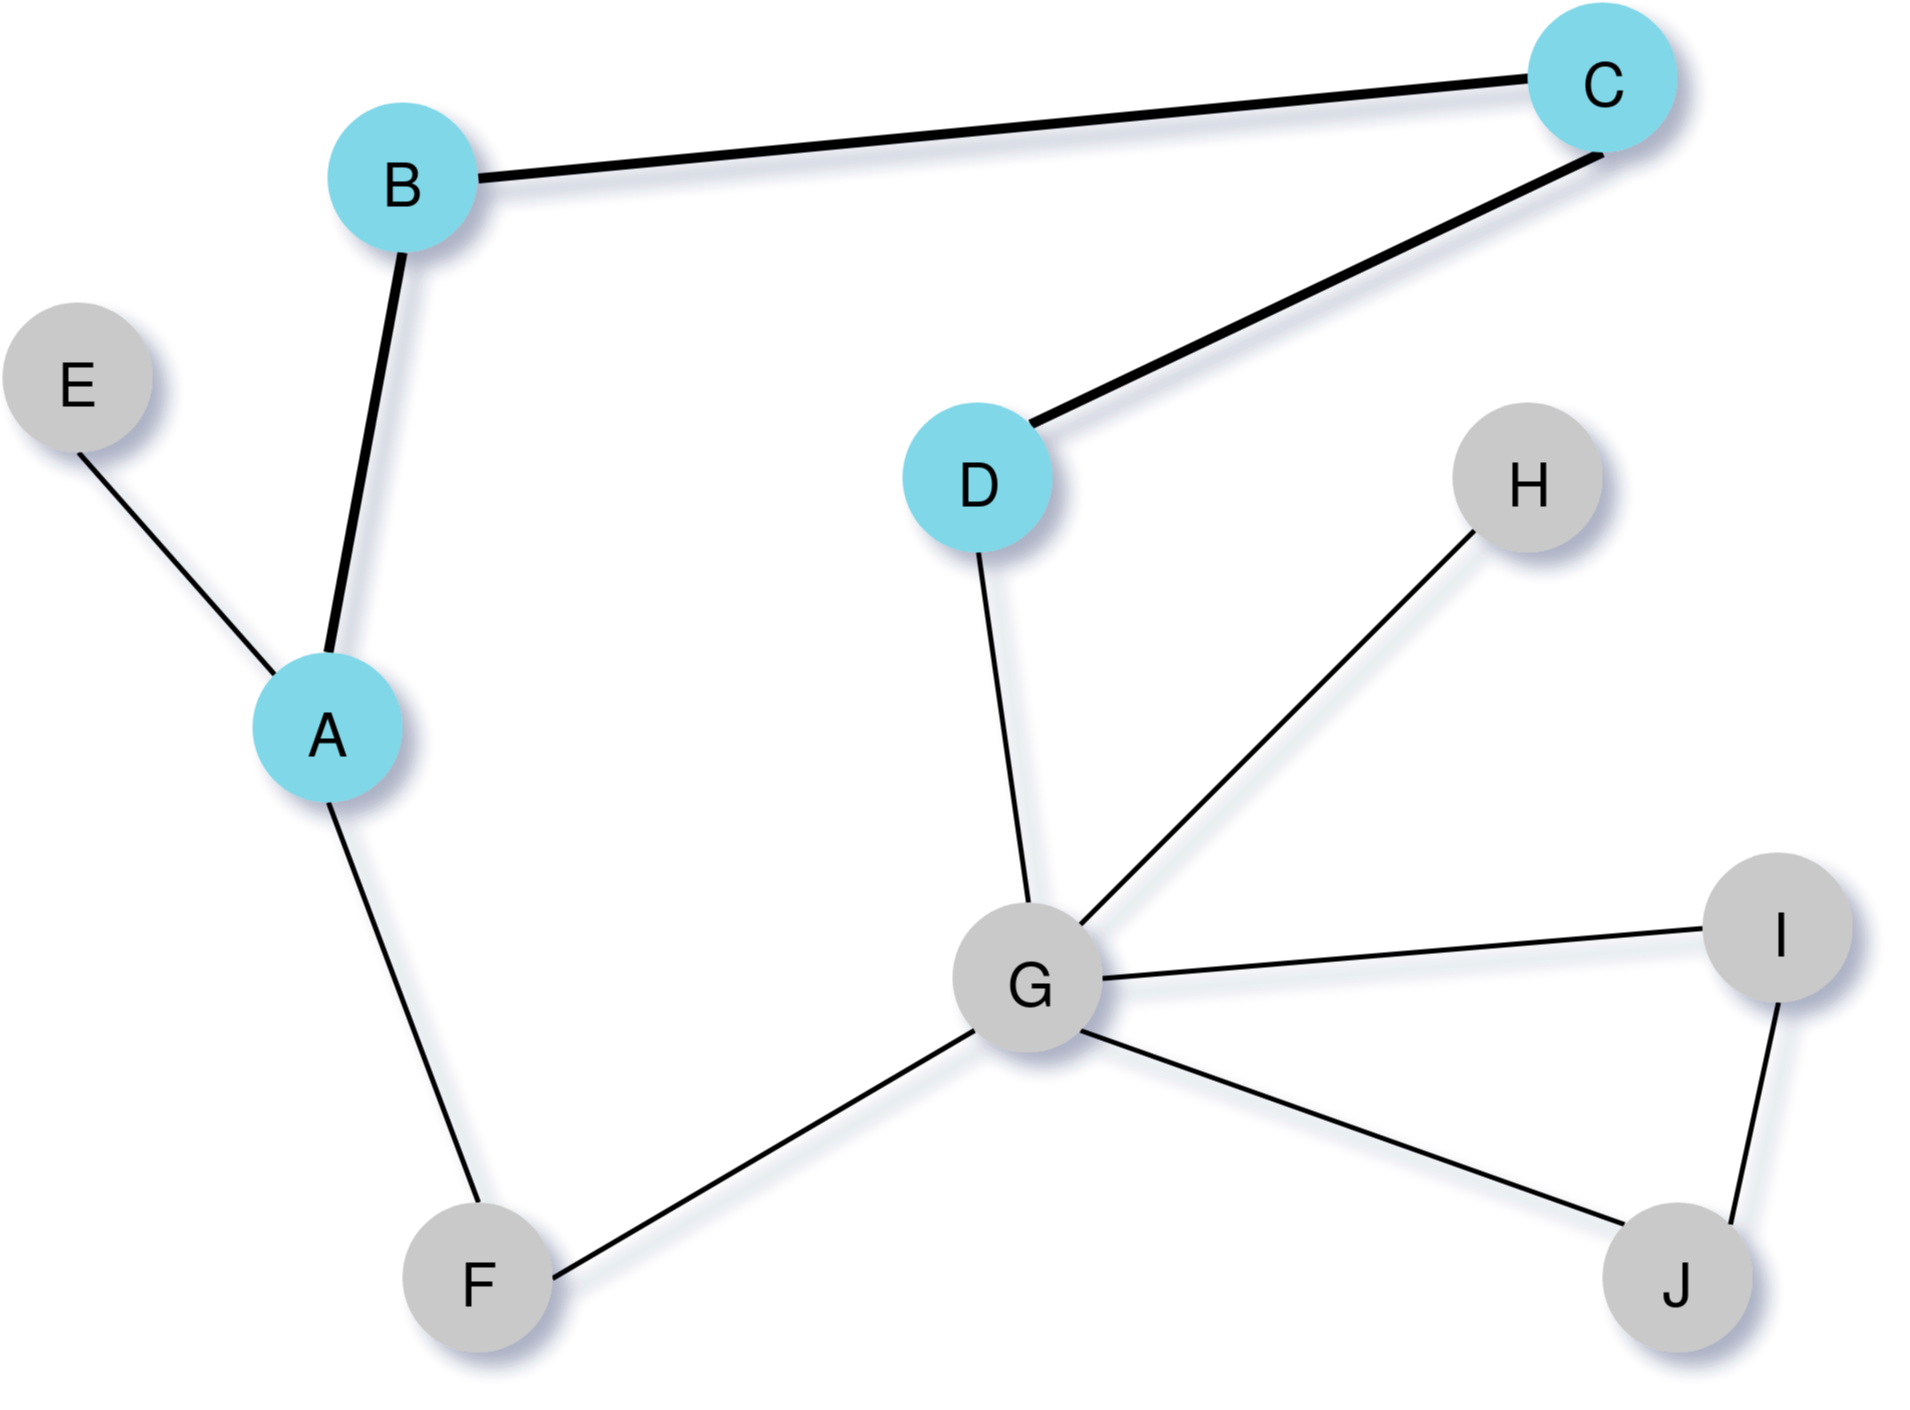
\includegraphics[width=0.55\textwidth]{introduction/images/mesh_network.png}
	\caption{A bais coverview of a lightning network, each node represent someone and each edge represents a channel between two people.}
	\label{fig:blockchain2}
\end{figure}

The name lightning network most likely a combination of lightning, as in lightning fast transactions. And network from the network that is formed by participants and their channels. One very useful feature of lightning network is that two parties do not need to have direct channel between them to be able to transact. Transactions can safely and atomically travel through the network via other participants, as long as there is a path between the two and there is enough funds in all the channels in between. 

\Subsection{Atomic swaps}
Another recent development in bitcoin and other cryptocurrency is atomic swaps. A regular swap can for example be two parties exchanging currencies. before this could be done in person, or via a trusted third-party handling all the transactions. Atomic swaps however is as the name implies atomic. Meaning that they either go through completely or no assets change hands at all, they are also completely trust-less meaning that you don't have to trust neither the other party or any third-party.

Just like lightning network atomic swaps use clever transaction scripts to achieve new functionality. Atomic swaps have been shown to be possible over lightning network, but it is ,mostly samll time projects and random writings on forums etc
Atomic swaps was first described by Tier Nolan in a post on \texttt{bitcointalk.org} on May 21, 2013


\Subsection{The goal of the project}
The goal of the project is to evaluate all the methods of atomic swaps available and compare them to a couple of different scenarios and use cases. Also I intned to become an expert in both atomic swaps and lightning network. 

